\documentclass[runningheads]{llncs}

% ---------------------------------------------------------------
% Include basic ECCV package
 
% TODO REVIEW: Insert your submission number below by replacing '*****'
% TODO FINAL: Comment out the following line for the camera-ready version
% \usepackage[review,year=****,ID=****]{****}
% TODO FINAL: Un-comment the following line for the camera-ready version
\usepackage{eccv}

% OPTIONAL: Un-comment the following line for a version which is easier to read
% on small portrait-orientation screens (e.g., mobile phones, or beside other windows)
%\usepackage[mobile]{****}


% ---------------------------------------------------------------
% Other packages

% Commonly used abbreviations (\eg, \ie, \etc, \cf, \etal, etc.)
\usepackage{eccvabbrv}
% Include other packages here, before hyperref.
\usepackage{graphicx}
\usepackage{booktabs}

% The "axessiblity" package can be found at: https://ctan.org/pkg/axessibility?lang=en
\usepackage[accsupp]{axessibility}  % Improves PDF readability for those with disabilities.


% ---------------------------------------------------------------
% Hyperref package

% It is strongly recommended to use hyperref, especially for the review version.
% Please disable hyperref *only* if you encounter grave issues.
% hyperref with option pagebackref eases the reviewers' job, but should be disabled for the final version.
%
% If you comment hyperref and then uncomment it, you should delete
% main.aux before re-running LaTeX.
% (Or just hit 'q' on the first LaTeX run, let it finish, and you
%  should be clear).

% TODO FINAL: Comment out the following line for the camera-ready version
% \usepackage[pagebackref,breaklinks,colorlinks,citecolor=eccvblue]{hyperref}
% TODO FINAL: Un-comment the following line for the camera-ready version
\usepackage{hyperref}

% Support for ORCID icon
\usepackage{orcidlink}


\begin{document}

% ---------------------------------------------------------------
% TODO REVIEW: Replace with your titlbluee
\title{Champ: Controllable and Consistent Human Image Animation with 3D Parametric Guidance} 

% TODO REVIEW: If the paper title is too long for the running head, you can set
% an abbreviated paper title here. If not, comment out.
\titlerunning{Champ: Controllable Human Image Animation w. 3D Parametric Guidance}

% TODO FINAL: Replace with your author list. 
% Include the authors' OCRID for the camera-ready version, if at all possible.
\author{Shenhao Zhu*\inst{1} \and
Junming Leo Chen*\inst{2} \and
Zuozhuo Dai\inst{3} \and
Qingkun Su\inst{3} \and \\
Yinghui Xu\inst{2} \and
Xun Cao\inst{1} \and 
Yao Yao\inst{1} \and
Hao Zhu$^\dag$\inst{1} \and
Siyu Zhu$^\dag$\inst{2} }

% TODO FINAL: Replace with an abbreviated list of authors.
\authorrunning{S. Zhu et al.}
% First names are abbreviated in the running head.
% If there are more than two authors, 'et al.' is used.

% TODO FINAL: Replace with your institution list.
\institute{Nanjing University, Nanjing, China \and
Fudan University, Shanghai, China \and
Alibaba Group, Hangzhou, China \\
\email{shenhaozhu@smail.nju.edu.cn, leochenjm@gmail.com, \\ \{caoxun, yaoyao, zh\}@nju.edu.cn, zuozhuo.dzz@alibaba-inc.com, \\ suqingkun@gmail.com, \{xuyinghui, siyuzhu\}@fudan.edu.cn}}

\maketitle

\input{sec/0_abs}
\let\thefootnote\relax\footnotetext{$^*$ These authors contributed equally to this work.}
\let\thefootnote\relax\footnotetext{ $^\dag$ Corresponding Author}
\vspace{-10pt}
\section{Introduction}
\label{sec:intro}
Autoregressive (AR) and diffusion models are two powerful paradigms for data distribution modeling. AR models, also known as the next token prediction approach, dominate language modeling and are considered central to the success of large language models (LLMs)~\cite{gpt1,gpt2,gpt3,llama1,llama2,llama3}. On the other hand, diffusion models~\cite{ddpm,dit,adm,edm}, or score-based generative models~\cite{songscore,lipman2023flow}, have emerged as the leading approach for visual generation, driving unprecedented progress in the era of visual content generation~\cite{sora,rombach2022high,li2023scaling}. 

\begin{figure}[t]
    \centering
    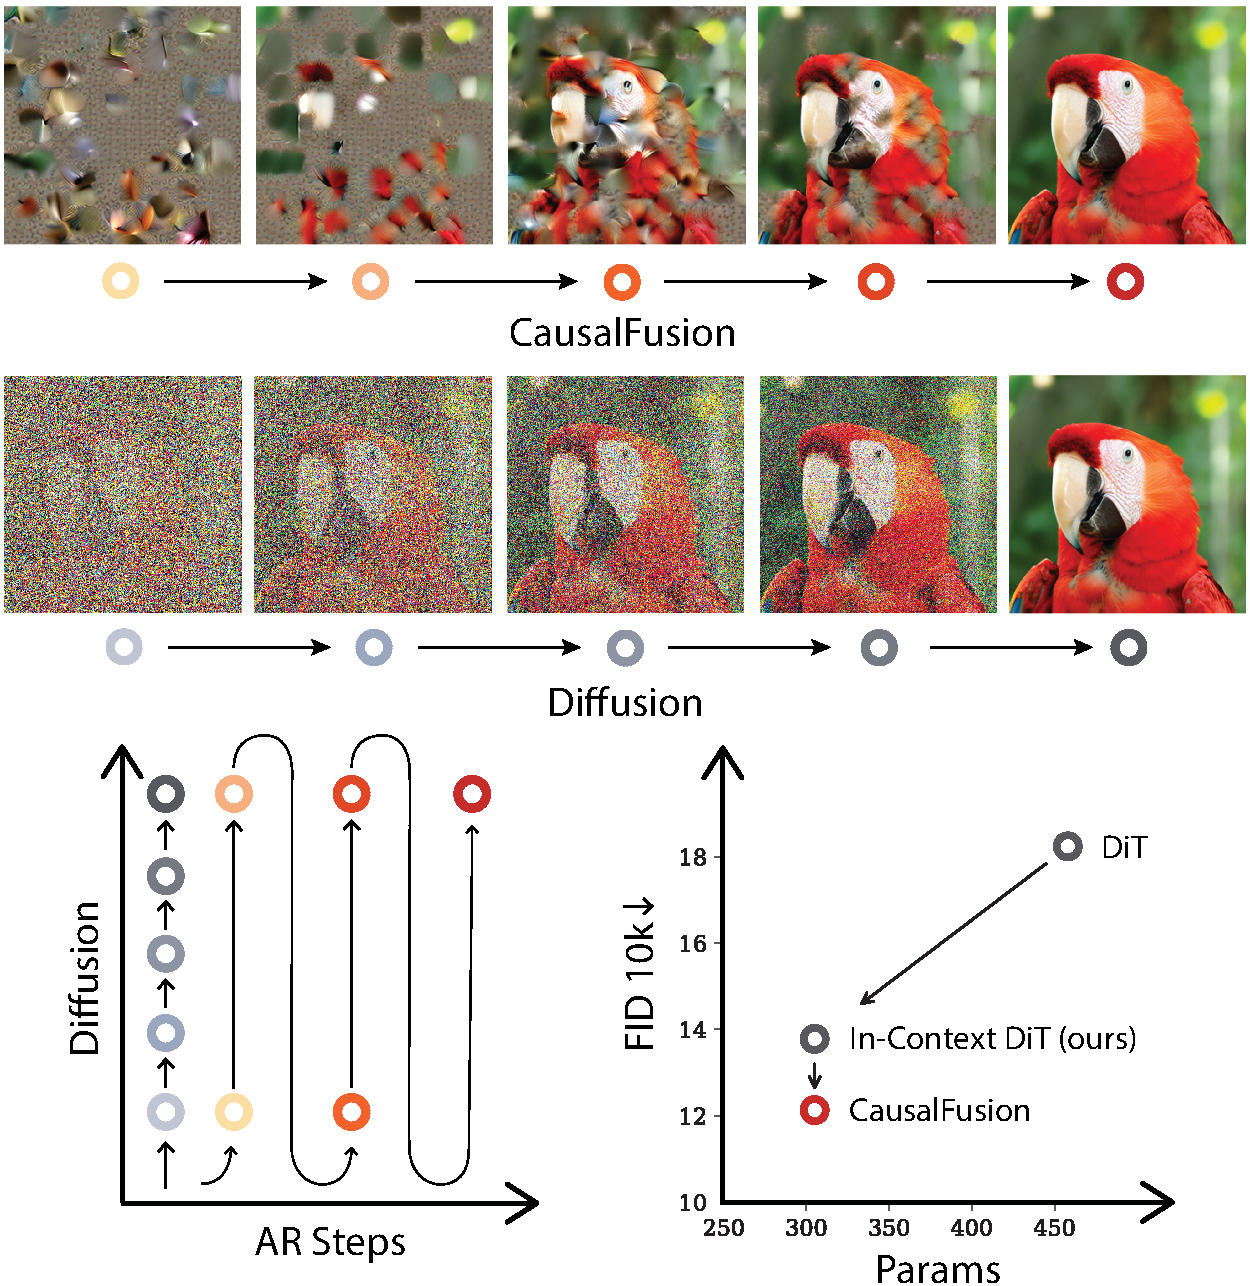
\includegraphics[width=1.0\textwidth,height=1.0\textwidth]{figs/casualfusion-teaser-v6.pdf} 
    \vspace*{-6mm}
    \caption{
    \textbf{Illustration of Dual-Factorization}. The arrow line indicates CausalFusion's generation path, moving from one state to the next by jointly generating along the sequential and noise-level dimension at each step. 
    Compared to DiT, our In-context DiT substantially improves results with fewer parameters. CausalFusion further enhances performance without changing the architecture or parameter count. Results were trained on IN1K for 240 epochs. CausalFusion adopts arbitrary AR steps for image generation, but each step only diffuses partial tokens, resulting in similar (or slightly lower) computational complexity.
    \vspace{-10pt}
    }
    \label{fig:dual-factorization}
\end{figure}


\begin{figure*}[t]
  \centering
  \begin{subfigure}{1.0\linewidth}
    \centering
    \includegraphics[width=\linewidth]{figs/figure2.pdf}
    \caption{Samples generated by CausalFusion-XL/2, ImageNet 512$\times$512, 800 epoch, DDPM 250 steps, CFG=4.0}
  \end{subfigure}
  \begin{subfigure}{1.0\linewidth}
    \centering
    \includegraphics[width=\linewidth]{figs/edit.pdf}
    \caption{\textbf{Zero-shot image editing} results generated by CausalFusion-XL/2, ImageNet 512$\times$512, 800 epoch. We first generate the original image (those on the left), then mask out its centre region, top-half, or bottom-half, and regenerate the image with new class conditions. Details are discussed in Sec \ref{sec:system}.}
  \end{subfigure}
  \caption{\textbf{Visualization results}. All samples are generated by models trained only on \textbf{ImageNet-1K class-conditional generation} task, demonstrating CausalFusion's zero-shot image manipulation ability. See more visualization results in Appendix~\ref{appendix:secD}.
  \vspace{-12pt}
  }
  \vspace{-6pt}
  \label{fig:vis1}
\end{figure*}

The intrinsic distinction between AR and diffusion models lies in their approach to data distribution factorization. AR models treat data as an ordered sequence, factorizing it along the sequential axis, where the probability of each token is conditioned on all preceding tokens. This factorization enables the AR paradigm to generalize effectively and efficiently across arbitrary number of tokens, making it well-suited for long-sequence reasoning and in-context generation. In contrast, diffusion models factorize data along the noise-level axis, where the tokens at each step are a refined (denoised) version of themselves from the previous step. As a result, the diffusion paradigm is generalizable to arbitrary number of data refinement steps, enabling iterative quality improvement with scaled inference compute. While AR and diffusion models each excel within their respective domains, their distinct factorization approaches reveal complementary potential. Although recent studies~\cite{transfusion,monoformer,dart} have attempted to integrate AR and diffusion within a single model, they typically treat these paradigms as separate modes, missing the potential benefits of jointly exploring them within a 2-D factorization plane.

To this end, we introduce \textbf{CausalFusion}, a flexible framework that integrates both sequential and noise-level data factorization to unify their advantages. The degree of factorization along these two axes—namely, the AR step and diffusion step—is adjustable, enabling {CausalFusion} to revert seamlessly to the traditional AR or diffusion paradigms at either extreme. To enhance its generality, CausalFusion is designed to predict \textit{any} number of tokens at \textit{any} AR step, with \textit{any} pre-defined sequence order and \textit{any} level of inference compute, thereby minimizing the inductive biases presented in existing generative models. As shown in Figure~\ref{fig:dual-factorization}, this approach provides a broad spectrum between the AR and diffusion paradigms, allowing smooth interpolation within two endpoints during both training and inference. 
Specifically, we explore CausalFusion in image generation and multimodal generation scenarios, where we observe that the level of training difficulties significantly influences the overall effectiveness of CausalFusion.

\textbf{Difficulties of generative tasks in CausalFusion:} Both AR and diffusion paradigms present unique challenges based on difficulties of their specific generative stages. In diffusion models, the effectiveness of training depends heavily on proper loss weighting across noise levels~\cite{ddpm,minsnr}, as higher noise levels are more difficult and usually provide more valuable signals than lower noise levels. Similarly, AR models are susceptible to error accumulation~\cite{bengio2015scheduled} as early-stage predictions are made with limited visible context, making them more error-prone. Optimizing CausalFusion thus requires balancing across these varying task difficulties to optimize training signal impact and ensure sufficient exploration across the entire factorization plane.

In this paper, we formally examine the difficulties of generative tasks within CausalFusion. We show that, in addition to the noise levels in diffusion and the amount of visible context in AR, the total number of AR steps, which controls the interpolation between AR and diffusion, also plays a critical role in shaping training difficulties. Driven by these factors, we develop a scalable and versatile model based on the CausalFusion framework. Starting from the DiT architecture~\cite{dit}, we gradually convert it into a decoder-only transformer compatible with existing AR models like GPT~\cite{gpt1,gpt2,gpt3} and LLaMA~\cite{llama1,llama2,llama3}. We provide insights on how to appropriately choose the number of AR steps during the training of CausalFusion models, and further introduce loss weighing along both the diffusion and AR axis to balance the impact of different generative stages. As shown in Figure~\ref{fig:dual-factorization} and ~\ref{fig:vis1}, our model achieves state-of-the-art performance on the ImageNet class-conditional generation benchmark, significantly outperforming DiT~\cite{dit} and enabling zero-shot image manipulations due to its AR nature. When pretraining on both text-to-image and image-to-text tasks, our model surpasses forced-fusion frameworks such as TransFusion~\cite{transfusion}, demonstrating the versatility of our CausalFusion framework.


We highlight our main contribution below:
\begin{itemize}
\item  We propose CausalFusion as the AR counterpart to DiT, achieving state-of-the-art results and enabling the unlimited token generation for in-context reasoning.
\item  We systematically study CausalFusion on the dual-factorization plane and identify key factors that improve the effectiveness of CausalFusion models.
\item  Compared with recent studies~\cite{transfusion}, CausalFusion enables a smooth, cohesive integration with language modeling for cross-modal generation and reasoning.
\end{itemize} 

% \begin{figure}[t]
%   \begin{minipage}{0.49\textwidth}
%      \centering
%     \includegraphics[width=1.0\textwidth]{fig/MLMF.png}
%     \caption{Multi-Layer Motion Fusion.}
%     \label{fig: frameselector_abalation}
    
%   \end{minipage}
%   \hfill
%    \begin{minipage}{0.48\textwidth}
%     \centering
%     \includegraphics[width=0.8\textwidth]{fig/SMPL.jpg}
%     \caption{Prametric Shape Alignment.}
%     \label{fig:Visualizedselected_frames}
%   \end{minipage}
% \vspace{-3mm}
% \end{figure}


\section{Related Work}
\label{sec:related_work}

\textbf{Diffusion Models for Image Generation.}
Diffusion-based models~\cite{balaji2022ediffi,huang2023composer,nichol2021glide,ramesh2022hierarchical,rombach2022high,saharia2022photorealistic} have rapidly emerged as a fundamental component in the domain of text-to-image generation, renowned for their capacity to yield highly promising generative outcomes. 
To address the considerable computational requirements inherent in diffusion models, the Latent Diffusion Model, as proposed in~\cite{rombach2022high} introduces a technique for denoising within the latent space.
This method not only enhances the computational efficiency of these models but also preserves their ability to generate high-fidelity images.
Moreover, in the endeavor to enhance control over visual generation, recent studies such as ControlNet~\cite{zhang2023adding}, T2I-Adapter~\cite{mou2023t2i}, and IP-Adapter~\cite{ye2023ip} have delved into the incorporation of supplementary encoder layers.
These layers facilitate the assimilation of control signals encompassing aspects such as pose, depth, and edge information, and even permit the utilization of images in conjunction with textual prompts.
This progression signifies a significant advancement towards more controlled and precise image generation, facilitating the creation of images characterized by not only superior quality but also enriched contextual accuracy and detail.


\textbf{Diffusion Models for Human Image Animation.}
The task of animating human images, a significant endeavor within the domain of video generation, aims to seamlessly create videos from one or multiple static images~\cite{chan2019everybody,ren2020deep,siarohin2019first,siarohin2021motion,yu2023bidirectionally,zhang2022exploring,zhao2022thin,yoon2021pose, sarkar2021neural, hu2023sherf, albahar2023humansgd, cao2023dreamavatar, prokudin2021smplpix, fu2022styleganhuman, jiang2023humangen}.
The recent advancements of diffusion models in the text-to-image domain have sparked interest in exploring their utility for animating human images.
PIDM~\cite{bhunia2023person} introduces a texture diffusion module that is specifically crafted to align the texture patterns of the source and target images closely, thereby enhancing the realism of the resultant animated output.
DreamPose~\cite{karras2023dreampose} capitalizes on the capabilities of the pre-trained Stable Diffusion model by incorporating both CLIP~\cite{radford2021learning} and VAE~\cite{kingma2013auto} for image encoding. 
It integrates these embeddings with an adapter. 
Similarly, DisCo~\cite{wang2023disco} innovatively segregates the control of pose and background using dual independent ControlNets~\cite{zhang2023adding}, providing finer control over the animation process. 
Animate Anyone~\cite{hu2023animate} utilizes a UNet-based ReferenceNet to extract features from reference images.
It includes pose information via a lightweight pose guider. Expanding on the principles introduced by AnimateDiff~\cite{guo2023animatediff}, Animate Anyone integrates a temporal layer into the denoising UNet to enhance temporal coherence.
MagicAnimate~\cite{xu2023magicanimate} follows a similar approach but employs a ControlNet tailored for DensePose \cite{guler2018dense} inputs instead of the more commonly used OpenPose~\cite{cao2017realtime} keypoints to provide more precise pose guidance.
This paper primarily builds upon esteemed diffusion-based methodologies and advances the optimization of appearance alignment and motion guidance mechanisms. 
This is achieved by introducing a 3D parametric model for geometric reconstruction of the reference image and motion modeling of the source video sequence.


\textbf{Pose Guidance in Human Image Animation.}
DWpose\cite{yang2023effective} stands out as an enhanced alternative to OpenPose\cite{cao2017realtime}, offering more accurate and expressive skeletons. 
This improvement has proven beneficial for diffusion models in generating higher quality images, with its adoption as a condition signal in various works\cite{feng2023dreamoving,hu2023animate}.
The work presented in DensePose~\cite{Guler2018DensePose} aims to establish dense correspondences between an RGB image and a surface-based representation.
The SMPL~\cite{SMPL:2015} model is a 3D model renowned for its realistic depiction of human bodies through skinning and blend shapes.
Its widespread adoption spans fields like human reconstruction\cite{he2021arch,alldieck2018video} and interaction with environments\cite{hassan2021populating,ma2020learning}. 
It also serves as essential ground truth for neural networks in pose and shape analysis\cite{lu2023dposer,mu2023actorsnerf}.
In this paper, we consider SMPL, the 3D parametric model, to reconstruct the poses as well as the shapes from the source video, and obtain more complete condition for appearance alignment and pose guidance.

\begin{figure}[t]
  \centering
  \includegraphics[width=0.95\linewidth]{fig/framework.jpg}
  \caption{The overview of our proposed approach. Given an input human image and a reference video depicting a motion sequence. We obtain the pose sequence corresponding to the reference image through Parametric Shape Alignment as 3D motion guidance. MLMF is employed to encode multi-layer 3D-related motion information. Referencenet and Temporal-attention ensure identity consistency and temporal coherence, respectively.}
  \vspace{-6mm}
  \label{fig:network}
\end{figure}
\section{Method}
%%%%%%%%% Figure: Overall framework
\begin{figure*}[t]
  \centering
   \includegraphics[width=0.85\linewidth]{figures/PoolFormer_overall_architecture.pdf}
   \vspace{-4mm}
   \caption{\textbf{(a) The overall framework of \modelname{}.} Similar to \cite{resnet, pvt, swin}, \modelname{} adopts hierarchical architecture with 4 stages. For a model with L \modelname{} blocks, stage [1, 2, 3, 4] have [L/6, L/6, L/2, L/6] blocks, respectively. The feature dimension $D_i$ of stage $i$ is shown in the figure. \textbf{(b) The architecture of \modelname{} block.} Compared with Transformer block, it replaces attention with extremely simple non-parametric operator, pooling, to conduct only basic token mixing.}
   \label{fig:overall_architecture}
\end{figure*}


%%%%%%%%% Algorithm: Pooling
\begin{algorithm}[t]
\caption{Pooling for PoolFormer, PyTorch-like Code}
\label{alg:code}
\definecolor{codeblue}{rgb}{0.25,0.5,0.5}
\definecolor{codekw}{rgb}{0.85, 0.18, 0.50}
\lstset{
  backgroundcolor=\color{white},
  basicstyle=\fontsize{7.5pt}{7.5pt}\ttfamily\selectfont,
  columns=fullflexible,
  breaklines=true,
  captionpos=b,
  commentstyle=\fontsize{7.5pt}{7.5pt}\color{codeblue},
  keywordstyle=\fontsize{7.5pt}{7.5pt}\color{codekw},
}
\begin{lstlisting}[language=python]
import torch.nn as nn

class Pooling(nn.Module):
    def __init__(self, pool_size=3):
        super().__init__()
        self.pool = nn.AvgPool2d(
            pool_size, stride=1, 
            padding=pool_size//2, 
            count_include_pad=False,
        )
    def forward(self, x):
        """
        [B, C, H, W] = x.shape
        Subtraction of the input itself is added 
        since the block already has a 
        residual connection.
        """
        return self.pool(x) - x
\end{lstlisting}
\end{algorithm}

\subsection{MetaFormer}
We present the core concept ``MetaFormer" for this work at first. As shown in Figure \ref{fig:first_figure}, abstracted from Transformers \cite{transformer}, 
MetaFormer is a general architecture where the token mixer is not specified while the other components are kept the same as Transformers. The input $I$ is first processed by input embedding, such as  patch embedding for ViTs \cite{vit},
\begin{equation}
    X = \mathrm{InputEmb}(I),
\end{equation}
where  $X \in \mathbb{R}^{N \times C}$ denotes the embedding tokens with sequence length $N$ and embedding dimension $C$. 


Then, embedding tokens are fed to repeated MetaFormer blocks, each of which includes two residual sub-blocks. Specifically, the first sub-block mainly contains a token mixer to communicate information among tokens and this sub-block can be expressed as
\begin{equation}
    Y = \mathrm{TokenMixer}(\mathrm{Norm}(X)) + X,
\end{equation}
where $\mathrm{Norm}(\cdot)$ denotes the normalization such as Layer Normalization \cite{layer_norm} or Batch Normalization \cite{batch_norm}; $\mathrm{TokenMixer}(\cdot)$ means a module mainly working for mixing token information. It is implemented by various attention mechanism in recent vision Transformer models  \cite{vit,refiner,t2t} or spatial MLP in MLP-like models \cite{mlp-mixer, resmlp}. Note that the main function of the token mixer is to propagate token information although some token mixers can also mix channels, like attention. 


The second sub-block primarily consists of a two-layered MLP with non-linear activation, 
\begin{equation}
    Z = \sigma(\mathrm{Norm}(Y)W_1)W_2 + Y,
\end{equation}
where $W_1 \in \mathbb{R}^{C \times rC}$ and $W_2 \in \mathbb{R}^{rC \times C}$ are learnable parameters with MLP expansion ratio $r$; $\sigma(\cdot)$ is a non-linear activation function, such as GELU \cite{gelu} or ReLU \cite{relu}. 

\myPara{Instantiations of MetaFormer} MetaFormer describes a general architecture 
% a general architecture that is powerful at solving computer vision tasks.  
with which different models can be obtained immediately by specifying the concrete design of the token mixers. 
As shown in Figure \ref{fig:first_figure}(a), if the token mixer is specified as attention or spatial MLP, MetaFormer then becomes a Transformer or MLP-like model respectively. 

\subsection{PoolFormer}
From the introduction of Transformers \cite{transformer}, lots of works attach much importance to the attention and focus on designing various attention-based token mixer components. In contrast, these works pay little attention to the general architecture, \ie, the MetaFormer.


In this work, we argue that this MetaFormer general architecture contributes mostly to the success of the recent Transformer and MLP-like models. 
To demonstrate it, we deliberately employ an embarrassingly simple operator, pooling, as the token mixer. This operator has no learnable parameters and it just makes each token averagely aggregate its nearby token features. 


Since this work is targeted at vision tasks,  we assume the input is in channel-first data format, \ie,  $T \in \mathbb{R}^{C \times H \times W}$. The pooling operator can be expressed as
\begin{equation}
\label{eq:pool}
    T'_{:, i, j} =  \frac{1}{K \times K} \sum_{p,q=1}^{K}T_{:, i+p-\frac{K+1}{2}, i+q-\frac{K+1}{2}} - T_{:, i, j},
\end{equation}
where $K$ is the pooling size. Since the MetaFormer block already has a residual connection, subtraction of the input itself is added in Equation (\ref{eq:pool}). The PyTorch-like code of the pooling is shown in Algorithm \ref{alg:code}.


As well known, self-attention and spatial MLP have computational complexity quadratic to the number of tokens to mix. Even worse, spatial MLPs bring much more parameters when handling longer sequences. As a result, self-attention and spatial MLPs usually can only process hundreds of tokens. In contrast, the pooling needs a computational complexity linear to the sequence length without any learnable parameters.  Thus, we take advantage of pooling by adopting a hierarchical structure similar to traditional CNNs \cite{alexnet, vgg, resnet} and recent hierarchical Transformer variants \cite{swin, pvt}. Figure \ref{fig:overall_architecture} shows the overall framework of PoolFormer. Specifically, PoolFormer has 4 stages with $\frac{H}{4} \times \frac{W}{4}$, $\frac{H}{8} \times \frac{W}{8}$, $\frac{H}{16} \times \frac{W}{16}$, and $\frac{H}{32} \times \frac{W}{32}$ tokens respectively, where $H$ and $W$ represent the width and height of the input image. There are two groups of embedding size: 1) small-sized models with embedding dimensions of 64, 128, 320, and 512 responding to the four stages; 2) medium-sized models with embedding dimensions 96, 192, 384, and 768. Assuming there are $L$ PoolFormer blocks in total, stages 1, 2, 3, and 4 will contain $L/6$, $L/6$, $L/2$, and $L/6$ PoolFormer blocks respectively. The MLP expansion ratio is set as 4. According to the above simple model scaling rule, we obtain 5 different model sizes of PoolFormer and their hyper-parameters are shown in Table \ref{tab:model}.


%%%%%%%%% Table: Model Configurations
\begin{table}[t]
\footnotesize
\centering
\setlength{\tabcolsep}{2pt}
% \scalebox{0.65}{\newcommand{\blockc}[4]{
$\begin{bmatrix}
	\begin{array}{l}
	R_1=#1 \\
	N_1=#2 \\
	E_1=#3 \\
	\end{array}
\end{bmatrix} \times #4$
}

\newcommand{\sblock}[3]{
$\begin{matrix}
E_{#1}=#2 \\
L_{#1}=#3 \\
\end{matrix}$
}

\newcommand{\poollayer}{
Pooling Size & \multicolumn{5}{c}{$3 \times 3$, stride 1}\\
\cline{4-9}
}

\newcommand{\stitle}[6]{
\multirow{5}{*}{#1} & \multirow{5}{*}{\scalebox{1}{$\frac{H}{#2}\times \frac{W}{#2}$}} & \multirow{2}{*}{\tabincell{c}{Patch \\ Embedding}} & Patch Size & \multicolumn{5}{c}{$#3 \times #3$, stride $#4$} \\
\cline{4-9}
    &    &    & Embed. Dim. & \multicolumn{3}{c|}{$#5$} & \multicolumn{2}{c}{$#6$} \\
\cline{3-9}
& & \multirow{3}{*}{\tabincell{c}{\modelname{}\\Block}} 
}

\begingroup
\renewcommand{\arraystretch}{1.1}
\begin{tabular}{c|c|c|c|c|c|c|c|c}
\toprule
  \multirow{2}{*}{Stage} & \multirow{2}{*}{\#Tokens} & \multicolumn{2}{c|}{\multirow{2}{*}{Layer Specification}} & \multicolumn{5}{c}{\modelname{}} \\
\cline{5-9}
 & & \multicolumn{2}{c|}{} & S12 & S24 & S36 & M36 & M48 \\
\whline
\stitle{1}{4}{7}{4}{64}{96}    & \poollayer
 & & & MLP Ratio & \multicolumn{5}{c}{4} \\
\cline{4-9}
 & & & \# Block & 2 & 4 & 6 & 6 & 8 \\
\hline
\stitle{2}{8}{3}{2}{128}{192}  & \poollayer
 & & & MLP Ratio & \multicolumn{5}{c}{4} \\
 \cline{4-9}
 & & & \# Block & 2 & 4 & 6 & 6 & 8 \\
\hline
\stitle{3}{16}{3}{2}{320}{384} & \poollayer
 & & & MLP Ratio & \multicolumn{5}{c}{4} \\
\cline{4-9}
 & & & \# Block & 6 & 12 & 18 & 18 & 24 \\
\hline
\stitle{4}{32}{3}{2}{512}{768} & \poollayer
 & & & MLP Ratio & \multicolumn{5}{c}{4} \\
 \cline{4-9}
 & & & \# Block & 2 & 4 & 6 & 6 & 8 \\
\hline
\multicolumn{4}{c|}{Parameters~(M)}& 11.9 & 21.4              &  30.8            &  56.1              &  73.4    \\
\hline
\multicolumn{4}{c|}{MACs~(G)}     & 1.8  &  3.4              &  5.0             &  8.8              &  11.6    \\
\bottomrule
\end{tabular}
\endgroup
}
\newcommand{\blockc}[4]{
$\begin{bmatrix}
	\begin{array}{l}
	R_1=#1 \\
	N_1=#2 \\
	E_1=#3 \\
	\end{array}
\end{bmatrix} \times #4$
}

\newcommand{\sblock}[3]{
$\begin{matrix}
E_{#1}=#2 \\
L_{#1}=#3 \\
\end{matrix}$
}

\newcommand{\poollayer}{
Pooling Size & \multicolumn{5}{c}{$3 \times 3$, stride 1}\\
\cline{4-9}
}

\newcommand{\stitle}[6]{
\multirow{5}{*}{#1} & \multirow{5}{*}{\scalebox{1}{$\frac{H}{#2}\times \frac{W}{#2}$}} & \multirow{2}{*}{\tabincell{c}{Patch \\ Embedding}} & Patch Size & \multicolumn{5}{c}{$#3 \times #3$, stride $#4$} \\
\cline{4-9}
    &    &    & Embed. Dim. & \multicolumn{3}{c|}{$#5$} & \multicolumn{2}{c}{$#6$} \\
\cline{3-9}
& & \multirow{3}{*}{\tabincell{c}{\modelname{}\\Block}} 
}

\begingroup
\renewcommand{\arraystretch}{1.1}
\begin{tabular}{c|c|c|c|c|c|c|c|c}
\toprule
  \multirow{2}{*}{Stage} & \multirow{2}{*}{\#Tokens} & \multicolumn{2}{c|}{\multirow{2}{*}{Layer Specification}} & \multicolumn{5}{c}{\modelname{}} \\
\cline{5-9}
 & & \multicolumn{2}{c|}{} & S12 & S24 & S36 & M36 & M48 \\
\whline
\stitle{1}{4}{7}{4}{64}{96}    & \poollayer
 & & & MLP Ratio & \multicolumn{5}{c}{4} \\
\cline{4-9}
 & & & \# Block & 2 & 4 & 6 & 6 & 8 \\
\hline
\stitle{2}{8}{3}{2}{128}{192}  & \poollayer
 & & & MLP Ratio & \multicolumn{5}{c}{4} \\
 \cline{4-9}
 & & & \# Block & 2 & 4 & 6 & 6 & 8 \\
\hline
\stitle{3}{16}{3}{2}{320}{384} & \poollayer
 & & & MLP Ratio & \multicolumn{5}{c}{4} \\
\cline{4-9}
 & & & \# Block & 6 & 12 & 18 & 18 & 24 \\
\hline
\stitle{4}{32}{3}{2}{512}{768} & \poollayer
 & & & MLP Ratio & \multicolumn{5}{c}{4} \\
 \cline{4-9}
 & & & \# Block & 2 & 4 & 6 & 6 & 8 \\
\hline
\multicolumn{4}{c|}{Parameters~(M)}& 11.9 & 21.4              &  30.8            &  56.1              &  73.4    \\
\hline
\multicolumn{4}{c|}{MACs~(G)}     & 1.8  &  3.4              &  5.0             &  8.8              &  11.6    \\
\bottomrule
\end{tabular}
\endgroup

\vspace{-3mm}
\caption{\textbf{ Configurations of different PoolFormer models.} There are two groups of embedding dimensions, \ie, small size with [64, 128, 320, 512] dimensions and medium size with [96, 196, 384, 768]. Notation ``S24" means the model is in small size of embedding dimensions with 24 PoolFormer blocks in total. The numbers of MACs are counted by \texttt{fvcore}\cite{fvcore} library.
}
\label{tab:model}
\vspace{-4mm}
\end{table}

% \begin{figure}[!t]
%   \centering
%   \includegraphics[width=1.0\linewidth]{fig/dataset.png}
%   \caption{Representative images of the proposed wild testing dataset.}
%   \label{fig:dataset}
%   \vspace{-5mm}
% \end{figure}

\section{Experiments}
\label{sec:exp}

\subsection{Implementations}
\textbf{Dataset.}
We have curated an in-the-wild dataset comprising approximately 5,000 high-fidelity authentic human videos sourced from reputable online repositories, encompassing a total of 1 million frames. 
The dataset is segmented as follows: Bilibili (2540 videos), Kuaishou (920 videos), Tiktok \& Youtube (1438 videos), and Xiaohongshu (430 videos). 
These videos feature individuals of varying ages, ethnicities, and genders, depicted in full-body, half-body, and close-up shots, set against diverse indoor and outdoor backdrops.
In order to enhance our model's capacity to analyze a wide range of human movements and attire, we have included footage of dancers showcasing various dance forms in diverse clothing styles. 
In contrast to existing datasets characterized by pristine backgrounds, our dataset capitalizes on the diversity and complexity of backgrounds to aid our model in effectively distinguishing the foreground human subjects from their surroundings.
To maintain fairness and align with established benchmarks in the field of image animation, the identical test set as utilized in MagicAnimate~\cite{xu2023magicanimate} has been employed for TikTok evaluation.

\begin{table}[!t]
\centering
\begin{tabular}{c|cccc|ccc}
\hline
Method          & L1 $\downarrow$ & PSNR $\uparrow$ & SSIM $\uparrow$ & LPIPS $\downarrow$  & FID-VID $\downarrow$ & FVD $\downarrow$ \\ \hline
MRAA  & 3.21E-04        & 29.39           & 0.672           & 0.296              & 54.47                           & 284.82           \\
DisCo             & 3.78E-04            & 29.03             & 0.668             & 0.292                            & 59.90                  & 292.80              \\
MagicAnimate  & 3.13E-04    & 29.16           & 0.714           & 0.239              & 21.75                          & 179.07           \\
Animate Anyone  & -            & 29.56             & 0.718             & 0.285                & -                                & 171.9              \\
Ours & 3.02E-04            & 29.84             & 0.773            & 0.235                             & 26.14                  & 170.20   \\
Ours*  & \textbf{2.94E-04}            & \textbf{29.91}             & \textbf{0.802}            & \textbf{0.234}                             & \textbf{21.07}                  & \textbf{160.82}         \\\hline
\end{tabular} 
\vspace{1mm}
\caption{Quantitative comparisons on Tiktok dataset.
* indicates that the proposed approach is fine-tuned on the Tiktok training dataset.}
\vspace{-4mm}
\label{tab:quantitative_tiktok}
\end{table}

\begin{figure*}[!t]
  \centering
  \includegraphics[width=\textwidth]{fig/qualitative_comparisons.png}
  \caption[]{Qualitative comparisons between our and the state-of-the-art approaches on TikTok and proposed unseen dataset.}
  \vspace{-4mm}
  \label{fig:qualitative_comparisons}
\end{figure*}

\textbf{Implementation.} 
Our experiments were facilitated by the computational power of 8 NVIDIA A100 GPUs. 
The training regimen is structured in two phases: initially, we processed individual video frames—sampling, resizing, and center-cropping them to a uniform resolution of 768x768 pixels. 
This stage spanned 60,000 steps with a batch size of 32. Subsequently, we dedicated attention to the temporal layer, training it over 20,000 steps with sequences of 24 frames and a reduced batch size of 8 to enhance temporal coherence. Both stages adhered to a learning rate of 1e-5.
During inference, to achieve continuity over extended sequences, we employed a temporal aggregation method, which facilitated the seamless integration of results from distinct batches, thereby generating longer video outputs. 

\begin{figure*}[!t]
  \centering
  \includegraphics[width=\textwidth]{fig/fig_comp_ubc.png}
  \caption[]{Qualitative comparisons between our and the state-of-the-art approaches on UBC fashion video datasets.}
  \label{fig:ubc_data}
\end{figure*}

\begin{figure*}[!t]
  \centering
  \includegraphics[width=\textwidth]{fig/fig_wild_results.png}
  \caption[]{More qualitative results of our approach on the proposed unseen dataset.}
  \vspace{-4mm}
  \label{fig:wild_data}
\end{figure*}

\subsection{Comparisons}
\textbf{Baselines.} We perform a comprehensive comparison with several state-of-the-art methods for human image animation: (1) MRAA~\cite{siarohin2021motion} is state-of-the-art GAN-based animation approaches, which estimate optical flow from driving sequences to warp the source image and then inpaint the occluded regions using GAN models. (2) DisCo~\cite{wang2023disco} is the state-of-the-art diffusion-based animation method that integrates disentangled condition modules for pose, human, and background into a pretrained diffusion model to implement human image animation. (3) MagicAnimate~\cite{xu2023magicanimate} and Animate Anyone~\cite{hu2023animate} are newer diffusion-based animation methods that employ more complex model structure and train on more general data which makes them perform quite well on TikTok dataset.
In all the qualitative (video and visual) comparative experiments, we employed the open-source implementation of Animate Anyone from MooreThreads\footnote{\tiny Animate Anyone: \url{https://github.com/MooreThreads/Moore-AnimateAnyone}} and MagicAnimate from the original authors\footnote{\tiny MagicAnimate: \url{https://github.com/magic-research/magic-animate}}. 
For all quantitative experimental comparisons, we directly referenced the relevant statistics from the original literature.

\begin{table}[!t]
\centering
\begin{tabular}{c|cccc}
    \hline
    Method          & PSNR $\uparrow$ & SSIM $\uparrow$ & LPIPS $\downarrow$ & FVD $\downarrow$ \\ \hline
    MRAA    & -          & 0.663           & 0.311           & 321.5                                   \\
    DisCo & 28.32          & 0.694           & 0.286          & 295.4    \\ 
    MagicAnimate & 29.14          & 0.713           & 0.235          & 193.6    \\ 
    Animate Anyone  & 28.86  &  0.727  & 0.242 & 199.2\\
    Ours  & \textbf{29.87}          & \textbf{0.806}           & \textbf{0.211}          & \textbf{173.5}\\ \hline
\end{tabular} 
\vspace{1mm}
\caption{Quantitative comparisons on proposed unseen dataset.}
\vspace{-4mm}
\label{tab:quantitative_wild}
\end{table}

\begin{table}[!t]
\centering
% \caption{Comparison of different methods on Image and Video metrics.}
\begin{tabular}{c|cccc|cc}
\hline
Method          & L1 $\downarrow$ & PSNR $\uparrow$ & SSIM $\uparrow$ & LPIPS $\downarrow$  & FID-VID $\downarrow$ & FVD $\downarrow$ \\ \hline
Ours (w/o. SMPL)  & 4.83E-04        & 28.57           & 0.672           & 0.296                  & 30.06                & 192.34          \\

Ours (w/o. geo.)  & 4.06E-04    & 28.78          & 0.714           & 0.276                        & 29.75                & 189.07           \\
Ours (w/o. skl.) & 3.76E-04            & 29.05            & 0.724             & 0.264            & 34.12                               & 184.24 \\
Ours & 3.02E-04          & 29.84           & 0.773            & 0.235          &  26.14                  & 170.20            \\\hline
\end{tabular}
\vspace{1mm}
\caption{Ablation study on different motion guidance.
``w/o. SMPL'' denotes a scenario where only the skeleton map is utilized as the motion condition.
``w/o. geo.'' indicates the model configuration that disregards geometric information, specifically depth and normal maps, as components of the motion condition.
``w/o. skl.'' describes the condition where the model solely relies on SMPL-derived inputs (including depth, normal, and semantic maps) for motion guidance.
``ours'' signifies the proposed approach that integrates both SMPL and skeleton derived motion condition.
}
\vspace{-4mm}
\label{tab:guidance_ablation}
\end{table}

\textbf{Evaluation metrics.} 
Our evaluation methodology adheres to the established metrics utilized in existing research literature.
Specifically, we assess both single-frame image quality and video fidelity. 
The evaluation of single-frame quality incorporates metrics such as the L1 error, Structural Similarity Index (SSIM)~\cite{wang2004image}, Learned Perceptual Image Patch Similarity (LPIPS)~\cite{zhang2018unreasonable}, and Peak Signal-to-Noise Ratio (PSNR)~\cite{5596999}. 
Video fidelity, on the other hand, is evaluated through the Frechet Inception Distance with Fréchet Video Distance (FID-FVD)~\cite{ijcai2019p276} and Fréchet Video Distance (FVD)~\cite{unterthiner2018towards}.

\textbf{Evaluation on benchmark dataset.}
Table~\ref{tab:quantitative_tiktok} presents a concise quantitative analysis of various methods evaluated on the TikTok dataset, focusing on key metrics such as L1 loss, PSNR, SSIM, LPIPS, FID-VID, and FVD. 
The proposed method, both in its original and fine-tuned (* indicated) forms, demonstrates superior performance across most metrics, particularly highlighting its effectiveness in achieving lower L1 loss, higher PSNR and SSIM values, and reduced LPIPS, FID-VID, and FVD scores. 
Notably, the fine-tuned version of our approach shows the best overall results, indicating the benefits of dataset-specific optimization. 
Figure~\ref{fig:qualitative_comparisons} and Figure~\ref{fig:ubc_data} provides additional qualitative comparison on such benchmark.

\textbf{Evaluation on Proposed Unseen Dataset.}
In order to further compare the robustness of various methods, distinct from datasets such as TikTok and UBC fashion that exhibit domain proximity, we have constructed a testing dataset comprising 100 high-fidelity authentic human videos sourced from online repositories.
These videos exhibit significant variations in the shape, pose, and appearance of the individuals depicted.
Figure~\ref{fig:wild_data} and Figure~\ref{fig:unseen_data} provides some qualitative comparison of the unseen dataset along with the statistical comparison presented in Table~\ref{tab:quantitative_wild}, collectively illustrate the efficacy of the proposed approach in generalizing to unseen domains.


\begin{table}[!t]
\centering
\begin{tabular}{c|cccc|cccc}
\hline
Method          & L1 $\downarrow$ & PSNR $\uparrow$ & SSIM $\uparrow$ & LPIPS $\downarrow$ &  FID-VID $\downarrow$ & FVD $\downarrow$ \\ \hline
w/o.  & 3.21E-04        & 29.44           & 0.752           & 0.248                      & 25.36                & 174.46           \\
w/.  & 3.02E-04           & 29.84             & 0.785            & 0.235                              & 21.28                  & 170.20             \\\hline
\end{tabular} 
\vspace{1mm}
\caption{Ablation study on guidance self-attention.}
\vspace{-4mm}
\label{tab:guidance_attention}
\end{table}

\begin{figure}[!t]
  \centering
  \includegraphics[width=1.0\linewidth]{fig/unseen.jpg}
  \caption{The qualitative comparison of animating unseen domain images.}
  \label{fig:unseen_data}
\end{figure}

\begin{figure}[!t]
  \centering
  \includegraphics[width=1.0\linewidth]{fig/cross_id.jpg}
  \caption{The demonstration of cross ID animation from the proposed approach.}
  \vspace{-4mm}
  \label{fig:cross_id}
\end{figure}

\begin{figure}[!t]
  \centering
  \includegraphics[width=1.0\linewidth]{fig/comp_sherf.png}
  \caption{Comparision between SHERF (left) and ours (right).}
  \vspace{-4mm}
  \label{fig:comp_sherf}
\end{figure}

\begin{figure}[!t]
  \centering
  \includegraphics[width=0.8\linewidth]{fig/shape_variance.jpg}
  \caption{The comparison on the shape variance data.}
  \label{fig:shape_variance}
\vspace{-4mm}  
\end{figure}



\textbf{Cross ID Animation.}
As shown in Figure~\ref{fig:cross_id}, a comparative analysis is conducted between our approach and state-of-the-art baseline methods for cross-identity animation, specifically focusing on the task of animating reference images through motion sequences derived from disparate videos.

\textbf{Multi-view Animation.}
Although our method may not match the direct rendering of 3D human representations for consistent novel views, we employ a sequence of SMPLs for multi-view consistent motion guidance and utilize generative models to achieve satisfactory multi-view results.  As shown in Figure~\ref{fig:comp_sherf}, we compare the results of our multi-view animation with a representative single-image to 3D human reconstruction method, SHERF~\cite{hu2023sherf}.

\subsection{Ablation Studies}
\textbf{Different Conditions from SMPL.}
As shown in Table~\ref{tab:guidance_ablation}, the statistics demonstrate that the full configuration of the proposed method (``ours'') obviously outperforms other variants in terms of image quality and fidelity, and video consistency and realism. 
The ablation components, ``w/o SMPL'', ``w/o geometry'', and ``w/o skeleton'', show progressively improved performance as more components are included.
Specifically, SMPL obviously brings more gains in PSNR (1.27 v.s. 0.48) and SSIM (0.10 v.s. 0.05) gains than a skeleton, which means better preserving the shape alignment and motion guidance.
Moreover, it is noteworthy that the incorporation of both the SMPL and skeleton models leads to additional improvements. 
Specifically, the skeleton model exhibits advantages in providing refined motion guidance for facial and hand regions.
Meanwhile, Figure~\ref{fig:ablation_motion} qualitative demonstrates the effectiveness of different conditions from SMPL.

\textbf{Guidance Self-Attention.}
Table~\ref{tab:guidance_attention} presents the findings of an ablation study conducted on guidance self-attention. 
The results indicate that the inclusion of guidance attention leads to superior performance compared to the absence of such attention, as evidenced by improvements across all evaluated metrics. 
As shown in Figure~\ref{fig:ablation_guidance}, we provide additional qualitative results of the guidance self-attention.

\begin{figure}[!t]
  \begin{minipage}{0.48\textwidth}
     \centering
    \includegraphics[width=1.0\textwidth]{fig/guidance_ablation.jpg}
    \caption{Ablation analysis on different motion conditions. geo. refers to the geometry. skl. is the skeleton condition.}
    \label{fig:ablation_motion}
    
  \end{minipage}
  \hfill
   \begin{minipage}{0.48\textwidth}
    \centering
    \includegraphics[width=0.9\textwidth]{fig/attention_ablation.jpg}
    \caption{Effect of guidance attention. w/. and w/o. indicate the guidance with and without self-attention.}
    \label{fig:ablation_guidance}
  \end{minipage}
\end{figure}

\textbf{Parametric Shape Alignment.}
As shown in Figure~\ref{fig:shape_variance},  we take an ablation study on shape parameter alignment between reference humans' SMPL model and driving videos' SMPL sequence. To highlight the effect, we use an individual with an extreme figure as the reference image and a common human dancing video as input. In comparison to other methods, our results from parametric shape alignment in the third row exhibit the most consistent shape and figure alignment with the reference image.

\textbf{Efficiency Analysis.}
Table~\ref{tab:efficiency} presents an efficiency analysis of our proposed approach, detailing the GPU memory requirements and time consumption for different steps, including parametric shape transfer, rendering per frame, and inference per frame.

\begin{table}[!t]
\centering
\begin{tabular}{c|ccccc}
\hline
Method          & GPU memory (GB) & & & & Time (sec) \\ \hline
Parametric shape transfer    &   3.24     & & & & 0.06 \\
Rendering (per frame) &  2.86    & & & & 0.07 \\
Inference (per frame)  & 19.83       & & & & 0.52 \\\hline
\end{tabular} 
\vspace{1mm}
\caption{Efficiency analysis of different steps of the proposed approach.} 
\label{tab:efficiency}
\vspace{-4mm}  
\end{table}

\subsection{Limitations and Future Works}
Despite the enhanced shape alignment capabilities and motion guidance offered by the human parametric SMPL model, its modeling capacity for faces and hands is limited. 
Consequently, the guidance effect for faces and hands does not match the efficacy of feature-based methods. This limitation underpins the incorporation of DWpose as an additional constraint for facial and hand modeling. 
As illustrated in Figure~\ref{fig:motion_guidance}, the self-attention mechanism further amplifies the saliency of faces and hands within the skeleton map. 
However, it is important to note that since SMPL and DWpose are solved independently, a potential discrepancy in consistency between them exists. 
Although this discrepancy did not manifest significantly in our experiments, it nonetheless introduces a potential source of error.
\section{Conclusion}
\label{sec:conclusion}

This paper introduces a novel approach to human image animation that integrates the SMPL 3D parametric human model with latent diffusion models, aiming to enhance pose alignment and motion guidance. 
By leveraging the unified representation of shape and pose variations offered by the SMPL model, along with depth, normal, and semantic maps, this method further improve the ability of capturing realistic human movements and shapes of previous techniques.
The inclusion of skeleton-based motion guidance and self-attention mechanisms for feature map integration further refines the animation process, enabling the creation of dynamic visual content that more accurately reflects human anatomy and movement. 
Experimental validation across various datasets confirms the effectiveness of this approach in producing high-quality human animations, showcasing its potential to advance digital content creation in fields requiring detailed and realistic human representations.


% \par\vfill\par
% Now we have reached the maximum length of an ECCV \ECCVyear{} submission (excluding references).
% References should start immediately after the main text, but can continue past p.\ 14 if needed.
% \clearpage  % TODO REVIEW/FINAL: This \clearpage needs to be removed from both review and camera-ready versions.


% ---- Bibliography ----
%
% BibTeX users should specify bibliography style 'splncs04'.
% References will then be sorted and formatted in the correct style.
%
\bibliographystyle{splncs04}
\bibliography{main}
\end{document}
